\documentclass[12pt,a4paper,article,english,firamath]{nsi}
\pagestyle{empty}
\newcommand{\truc}{4.5cm}
\geometry{margin=.9cm}
\begin{document}
\LARGE
\begin{center}
\begin{tabular}{|c|c|}
\hline
\rowcolor{UGLiOrange}\textbf{\color{white}Processus élu} & \textbf{\color{white}Graphe d'allocation des ressources} \\
\hline
 & 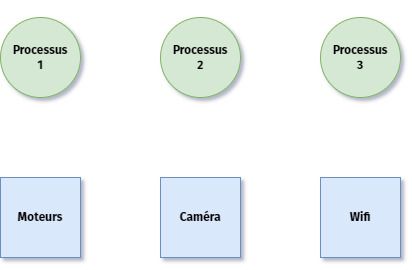
\includegraphics[width=\truc]{img/d6.png} \\
\hline
 & 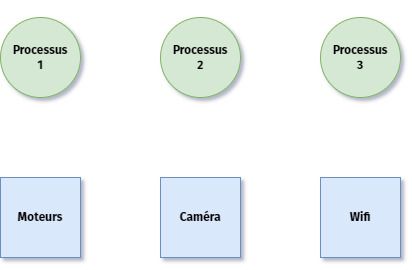
\includegraphics[width=\truc]{img/d6.png} \\
\hline
 & 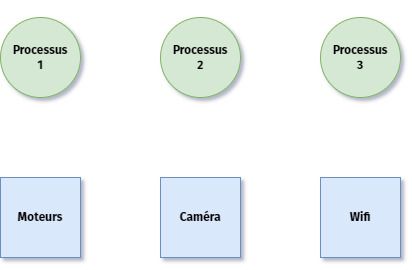
\includegraphics[width=\truc]{img/d6.png} \\
\hline
 & 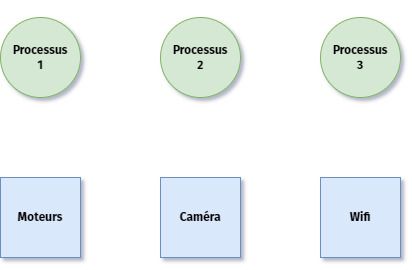
\includegraphics[width=\truc]{img/d6.png} \\
\hline
 & 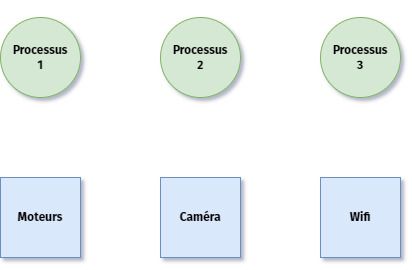
\includegraphics[width=\truc]{img/d6.png} \\
\hline
 & 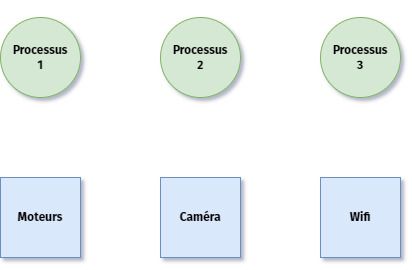
\includegraphics[width=\truc]{img/d6.png} \\
\hline
 & 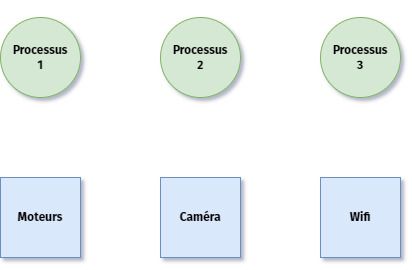
\includegraphics[width=\truc]{img/d6.png} \\
\hline
 & 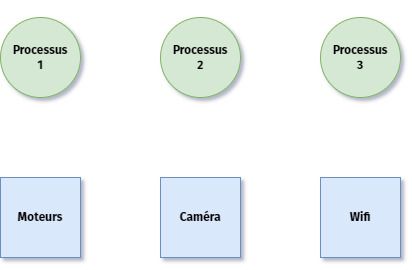
\includegraphics[width=\truc]{img/d6.png} \\
\hline
 \end{tabular}
\end{center}
\newpage

\begin{center}
\begin{tabular}{|c|c|}
\hline
\rowcolor{UGLiOrange}\textbf{\color{white}Processus élu} & \textbf{\color{white}Graphe d'allocation des ressources} \\
\hline
 & 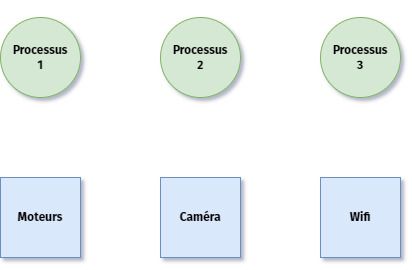
\includegraphics[width=\truc]{img/d6.png} \\
\hline
 & 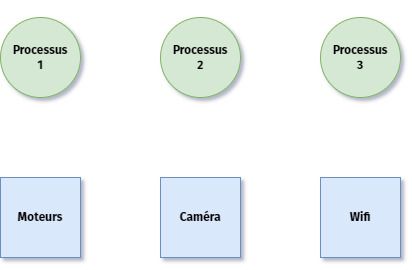
\includegraphics[width=\truc]{img/d6.png} \\
\hline
 & 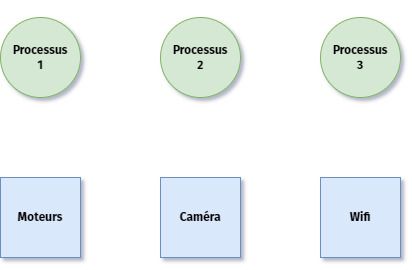
\includegraphics[width=\truc]{img/d6.png} \\
\hline
 & 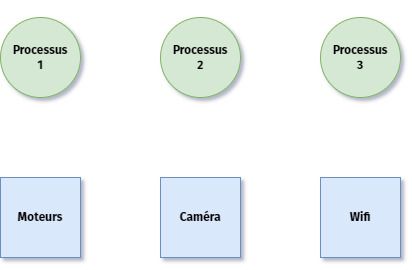
\includegraphics[width=\truc]{img/d6.png} \\
\hline
 & 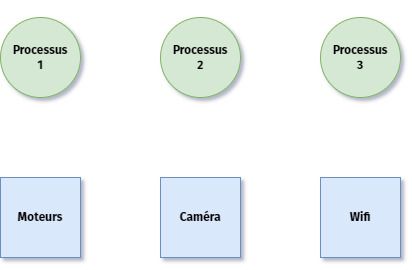
\includegraphics[width=\truc]{img/d6.png} \\
\hline
 & 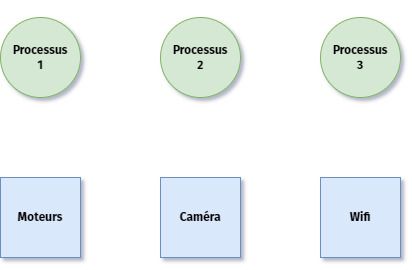
\includegraphics[width=\truc]{img/d6.png} \\
\hline
 & 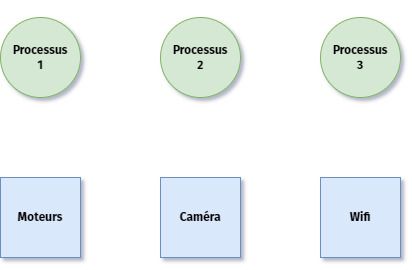
\includegraphics[width=\truc]{img/d6.png} \\
\hline
 & 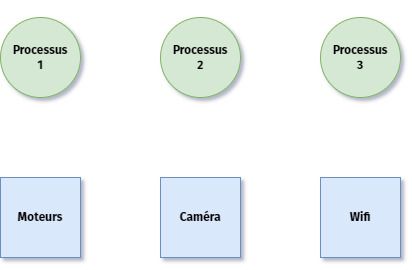
\includegraphics[width=\truc]{img/d6.png} \\
\hline
 \end{tabular}
\end{center}
\newpage

\begin{center}
\begin{tabular}{|c|c|}
\hline
\rowcolor{UGLiOrange}\textbf{\color{white}Processus élu} & \textbf{\color{white}Graphe d'allocation des ressources} \\
\hline
 & 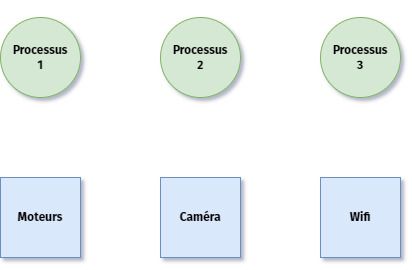
\includegraphics[width=\truc]{img/d6.png} \\
\hline
 & 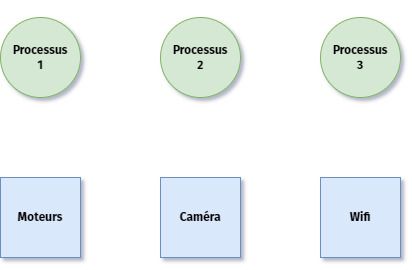
\includegraphics[width=\truc]{img/d6.png} \\
\hline
 & 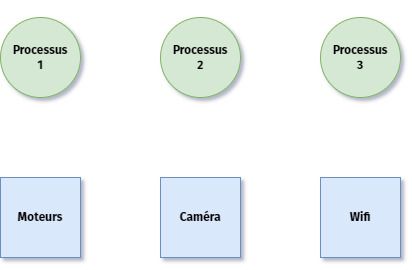
\includegraphics[width=\truc]{img/d6.png} \\
\hline
 & 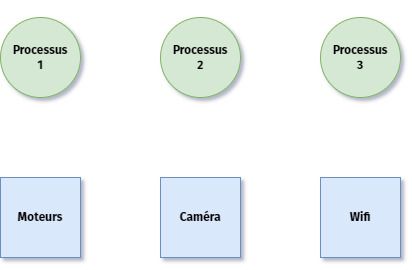
\includegraphics[width=\truc]{img/d6.png} \\
\hline
 & 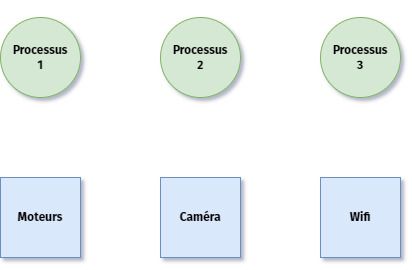
\includegraphics[width=\truc]{img/d6.png} \\
\hline
 & 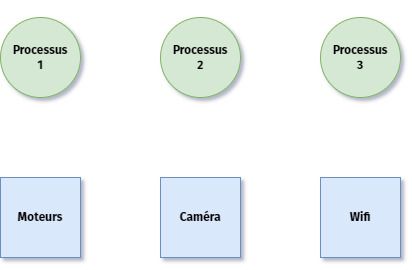
\includegraphics[width=\truc]{img/d6.png} \\
\hline
 & 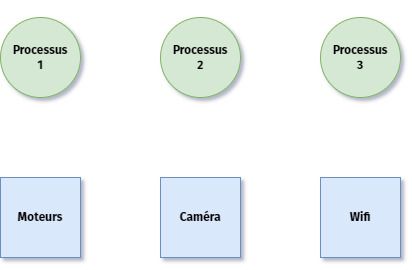
\includegraphics[width=\truc]{img/d6.png} \\
\hline
 & 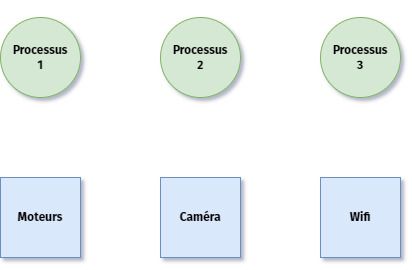
\includegraphics[width=\truc]{img/d6.png} \\
\hline
 \end{tabular}
\end{center}
\newpage




\begin{center}
\begin{tabular}{|c|}
\hline
\rowcolor{UGLiOrange} \textbf{\color{white}Processus 1 }\\
\hline
demande \textbf{R1} (moteurs) \\
\hline
demande \textbf{R2} (wifi) \\
\hline
se déplace et transmet sa position\\
\hline
libère \textbf{R1} (moteurs) \\
\hline
libère \textbf{R2} (wifi) \\
\hline
\end{tabular}
\end{center}
\ \\
\begin{center}
\begin{tabular}{|c|}
\hline
\rowcolor{UGLiOrange} \textbf{\color{white}Processus 2}\\
\hline
demande \textbf{R2} (wifi) \\
\hline
 demande \textbf{R3} (caméra) \\
\hline
prend une photo et la transmet\\
\hline
 libère \textbf{R2} (wifi)   \\
\hline
 libère \textbf{R3} (caméra)   \\
\hline
\end{tabular}
\end{center}
\ \\
\begin{center}
\begin{tabular}{|c|}
\hline
\rowcolor{UGLiOrange}\textbf{\color{white}Processus 3} \\
\hline
 demande \textbf{R3} (caméra) \\
\hline
demande \textbf{R1} (moteurs) \\
\hline
effectue des tests caméra/moteur\\
\hline
libère \textbf{R3} (caméra)  \\
\hline
libère \textbf{R1} (moteurs)  \\
\hline
\end{tabular}
\end{center}


\end{document}
\pagestyle{empty}
\newcommand{\truc}{4.5cm}
\begin{document}
\LARGE
\begin{center}
\begin{tabular}{|c|c|}
\hline
\rowcolor{UGLiOrange}\textbf{\color{white}Processus élu} & \textbf{\color{white}Graphe d'allocation des ressources} \\
\hline
 & 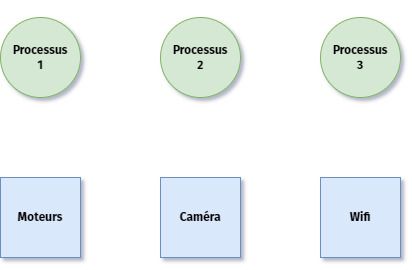
\includegraphics[width=\truc]{img/d6.png} \\
\hline
 & 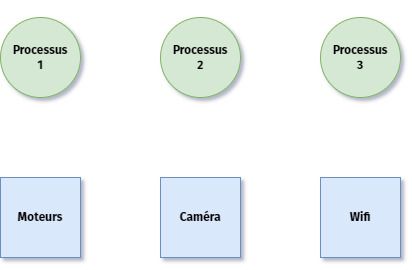
\includegraphics[width=\truc]{img/d6.png} \\
\hline
 & 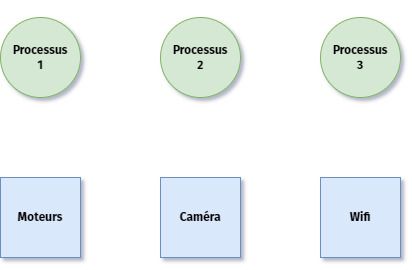
\includegraphics[width=\truc]{img/d6.png} \\
\hline
 & 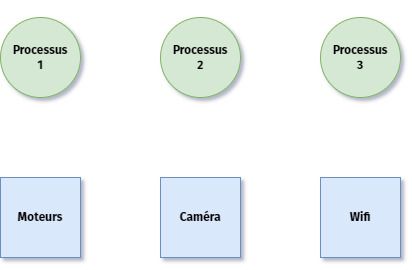
\includegraphics[width=\truc]{img/d6.png} \\
\hline
 & 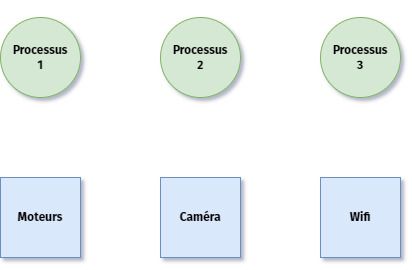
\includegraphics[width=\truc]{img/d6.png} \\
\hline
 & 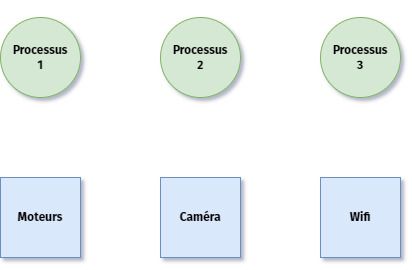
\includegraphics[width=\truc]{img/d6.png} \\
\hline
 & 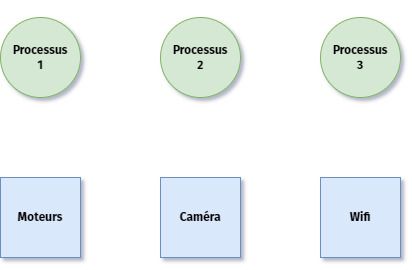
\includegraphics[width=\truc]{img/d6.png} \\
\hline
 & 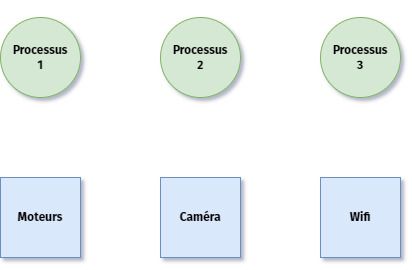
\includegraphics[width=\truc]{img/d6.png} \\
\hline
 \end{tabular}
\end{center}
\newpage

\begin{center}
\begin{tabular}{|c|c|}
\hline
\rowcolor{UGLiOrange}\textbf{\color{white}Processus élu} & \textbf{\color{white}Graphe d'allocation des ressources} \\
\hline
 & 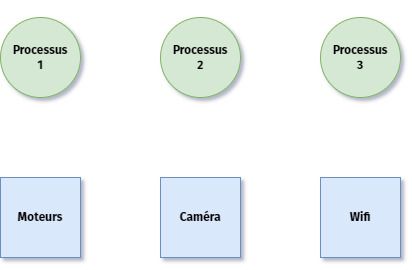
\includegraphics[width=\truc]{img/d6.png} \\
\hline
 & 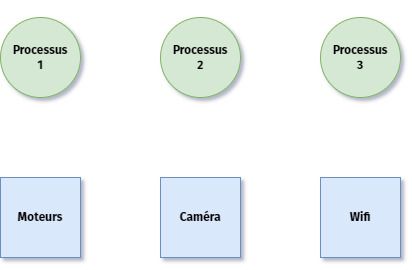
\includegraphics[width=\truc]{img/d6.png} \\
\hline
 & 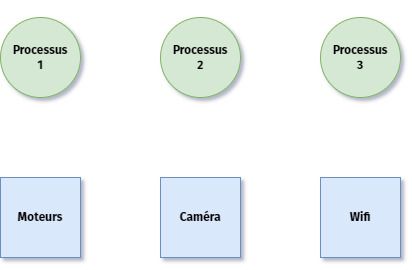
\includegraphics[width=\truc]{img/d6.png} \\
\hline
 & 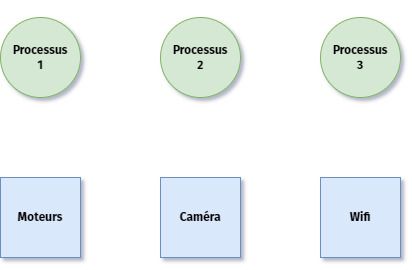
\includegraphics[width=\truc]{img/d6.png} \\
\hline
 & 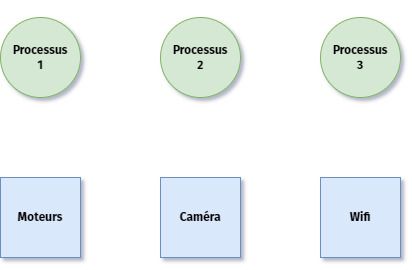
\includegraphics[width=\truc]{img/d6.png} \\
\hline
 & 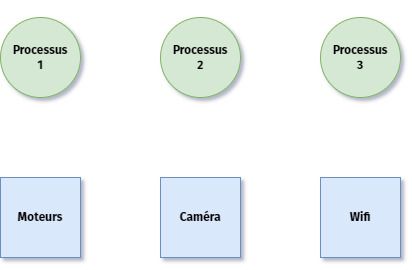
\includegraphics[width=\truc]{img/d6.png} \\
\hline
 & 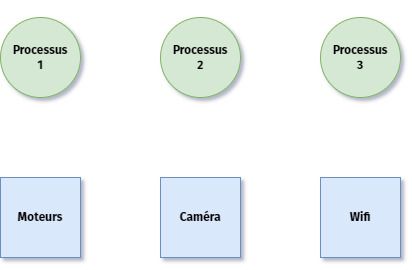
\includegraphics[width=\truc]{img/d6.png} \\
\hline
 & 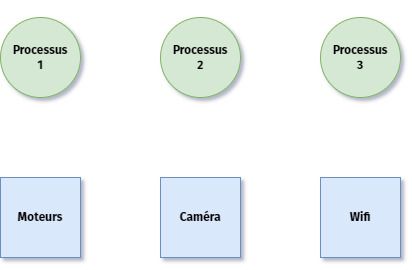
\includegraphics[width=\truc]{img/d6.png} \\
\hline
 \end{tabular}
\end{center}
\newpage

\begin{center}
\begin{tabular}{|c|c|}
\hline
\rowcolor{UGLiOrange}\textbf{\color{white}Processus élu} & \textbf{\color{white}Graphe d'allocation des ressources} \\
\hline
 & 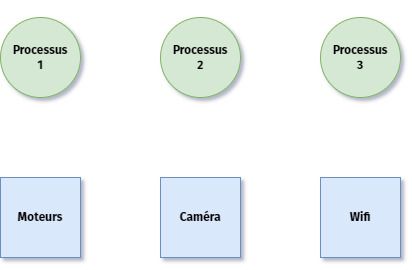
\includegraphics[width=\truc]{img/d6.png} \\
\hline
 & 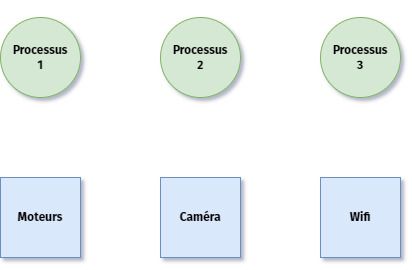
\includegraphics[width=\truc]{img/d6.png} \\
\hline
 & 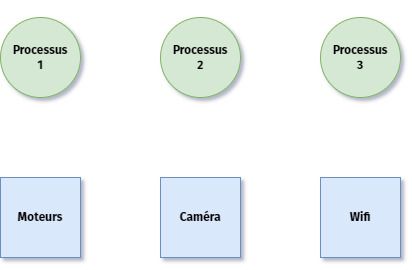
\includegraphics[width=\truc]{img/d6.png} \\
\hline
 & 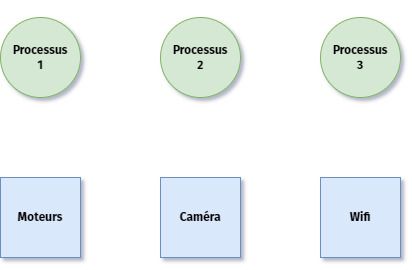
\includegraphics[width=\truc]{img/d6.png} \\
\hline
 & 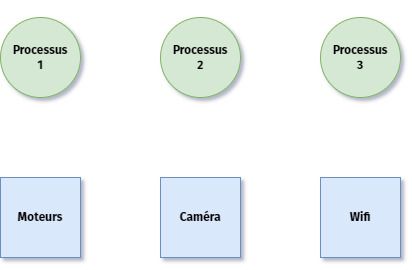
\includegraphics[width=\truc]{img/d6.png} \\
\hline
 & 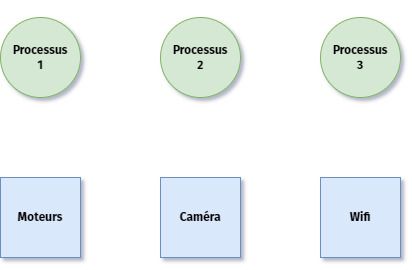
\includegraphics[width=\truc]{img/d6.png} \\
\hline
 & 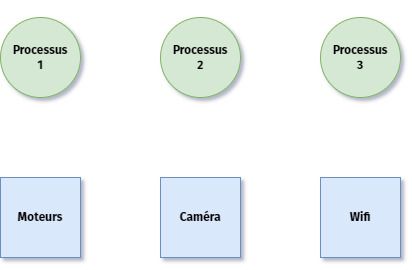
\includegraphics[width=\truc]{img/d6.png} \\
\hline
 & 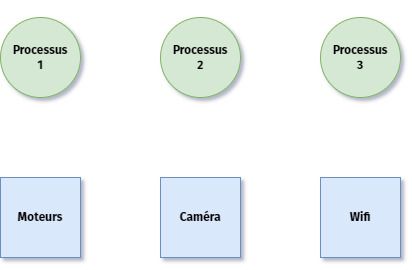
\includegraphics[width=\truc]{img/d6.png} \\
\hline
 \end{tabular}
\end{center}
\newpage




\begin{center}
\begin{tabular}{|c|}
\hline
\rowcolor{UGLiOrange} \textbf{\color{white}Processus 1 }\\
\hline
demande \textbf{R1} (moteurs) \\
\hline
demande \textbf{R2} (wifi) \\
\hline
se déplace et transmet sa position\\
\hline
libère \textbf{R1} (moteurs) \\
\hline
libère \textbf{R2} (wifi) \\
\hline
\end{tabular}
\end{center}
\ \\
\begin{center}
\begin{tabular}{|c|}
\hline
\rowcolor{UGLiOrange} \textbf{\color{white}Processus 2}\\
\hline
demande \textbf{R2} (wifi) \\
\hline
 demande \textbf{R3} (caméra) \\
\hline
prend une photo et la transmet\\
\hline
 libère \textbf{R2} (wifi)   \\
\hline
 libère \textbf{R3} (caméra)   \\
\hline
\end{tabular}
\end{center}
\ \\
\begin{center}
\begin{tabular}{|c|}
\hline
\rowcolor{UGLiOrange}\textbf{\color{white}Processus 3} \\
\hline
 demande \textbf{R3} (caméra) \\
\hline
demande \textbf{R1} (moteurs) \\
\hline
effectue des tests caméra/moteur\\
\hline
libère \textbf{R3} (caméra)  \\
\hline
libère \textbf{R1} (moteurs)  \\
\hline
\end{tabular}
\end{center}


\end{document}